\documentclass[10pt]{beamer}

%\usetheme{metropolis}
%\usetheme{AnnArbor}
\usetheme[progressbar=frametitle]{metropolis}
%\usecolortheme{beaver}
\usepackage{appendixnumberbeamer}

\usepackage{booktabs}
\usepackage[scale=2]{ccicons}

\usepackage{pgfplots}
\usepgfplotslibrary{dateplot}

%\usepackage[brazil]{babel}
\usepackage{xspace}
\usepackage{algorithm2e} % AAB inserido
\newcommand{\themename}{\textbf{\textsc{metropolis}}\xspace}
%\usepackage[brazil]{babel}  % AAB
\usepackage{bibentry}       % AAB
\usepackage{amsmath, bm}    % AAB
\usepackage{tikz}           % AAB
\usetikzlibrary{chains,fit,shapes} % AAB 
\usepackage[detect-weight=true, binary-units=true]{siunitx}
%\usepackage{siunitx}        % AAB inserido    
\usetikzlibrary{shapes,arrows,shadows}  % AAB inserido
%\usepackage[utf8]{inputenc}                  % AAB inserido
                                              % AAB inserido
\usepackage[caption=false,font=normalsize,labelfont=sf,textfont=sf]{subfig}
%\usepackage[caption=false,font=footnotesize]{subfig}
%
%\addto\captionsportuguese{
%\renewcommand{\figurename}{Fig.}
%\renewcommand{\tablename}{Tab.}
%}% AAB Inserido
\DeclareMathOperator{\traco}{tr} %AAB
\graphicspath{{../Dissertacao/figuras/}}        % AAB - caminho das figuras
%\graphicspath{{../Images/PDF/}}                 % AAB - caminho das figuras (recomendável) 


\title{Fusion of Evidences in Intensity Channels for Edge Detection in PolSAR Images}
\subtitle{Ongoing researches}
\date{}
\author{Dr. Anderson Adaime de Borba - IBMEC -- SP -- BR\\
        Dr. Mauricio Marengoni -- UFMG -- BR\\
        Dr. Alejandro Frery - Victoria University of Wellington -- NZ} 
\institute{SP-MAR-2021}
\begin{document}
\maketitle
\begin{frame}[fragile]{SAR -- PolSAR}
\centering
       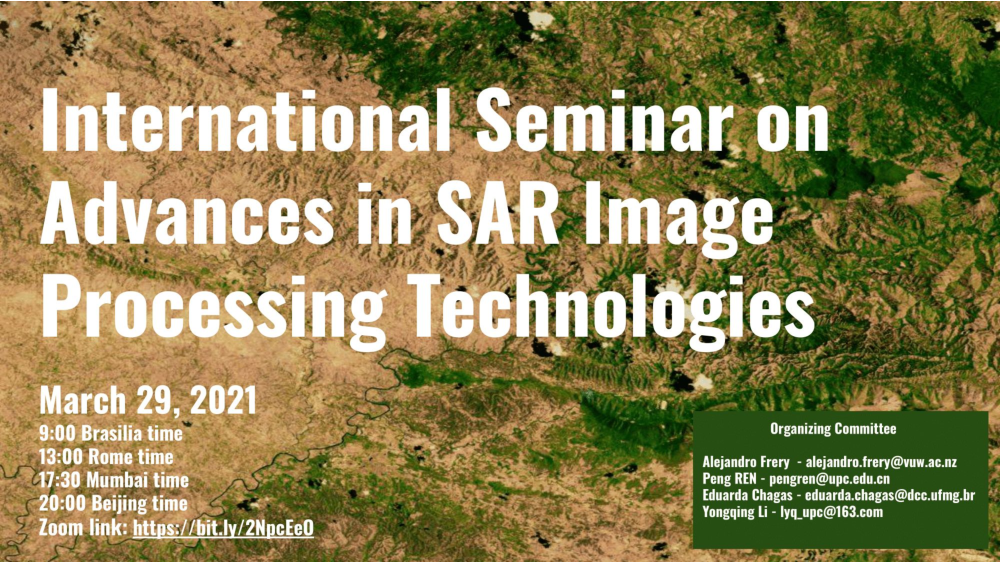
\includegraphics[width=1.0\linewidth]{sem_int_2021_03}
\end{frame}
%
\begin{frame}[fragile]{Inter-institutional cooperation projects}
\centering{
\includegraphics[width=6cm]{logo_uni_wellington}\\
\includegraphics[width=6cm]{logo_ufmg}\\
\includegraphics[width=6cm]{logo_ibmec1}\\}
\end{frame}
%
%\begin{frame}{Índice}
%  \setbeamertemplate{section in toc}[sections numbered]
%  \tableofcontents[hideallsubsections]
%\end{frame}
%	
\begin{frame}[fragile]{Database (PolSAR Image)}
\begin{alertblock}{PolSAR Data}
\begin{table}[hbt]
\scriptsize
	\centering
	\caption{Information from the PolSAR system.}
\begin{tabular}{@{}lccc@{}} \toprule
	Polarization & hh  & hv & vv \\ \midrule
	hh & $\sigma_\text{hh}$ & $\Re\big(\text{Cov}(\text{hh}, \text{hv})\big) + \Im\big(\text{Cov}(\text{hh}, \text{hv})\big)\hat{\jmath}$  & $\Re\big(\text{Cov}(\text{hh}, \text{vv})\big) + \Im\big(\text{Cov}(\text{hh}, \text{vv})\big)\hat{\jmath}$\\ 
	hv &- &$\sigma_\text{hv}$ & $ \Re\big(\text{Cov}(\text{hv}, \text{vv})\big)+ \Im\big(\text{Cov}(\text{hv}, \text{vv})\big)\hat{\jmath}$\\ 
	vv &- & -&$\sigma_\text{vv}$ \\ \bottomrule 
\end{tabular}\label{tab:sistema_polsar}
\end{table}
\begin{table}[hbt]	
	\centering
	\caption{PolSAR intensity channels.}
\begin{tabular}{@{}lcc@{}} \toprule
	 $\text{C}_1$ &$\text{C}_2$&$\text{C}_3$ \\ \midrule
	$\sigma_\text{hh}$&$\sigma_\text{hv}$&$\sigma_\text{vv}$\\ \bottomrule
\end{tabular}\label{tab:canais}
\end{table}
\end{alertblock}
\end{frame}
%
\begin{frame}[fragile]{Image channels.}
   \begin{figure}[hbt]
\minipage{0.35\textwidth}
  \includegraphics[width=\linewidth]{sf_hh.pdf}
\endminipage
\minipage{0.35\textwidth}
	\includegraphics[width=\linewidth]{sf_vh.pdf}
\endminipage
\centering
\minipage{0.35\textwidth}
	\includegraphics[width=\linewidth]{sf_vv.pdf}
\endminipage
	\caption{PolSAR images with polarization hh, hv e vv.}\label{fig:sf_hh_hv_vv}
\end{figure}
\end{frame}
%
\begin{frame}[fragile]{General Idea.}
\begin{alertblock}{Fusion scheme}
%\begin{itemize}
%\item Parte II - Para cada $\bm{\widehat\imath}_t$
\pgfdeclarelayer{background}
\pgfdeclarelayer{foreground}
\pgfsetlayers{background,main,foreground}
%
\pgfdeclarelayer{background}
\pgfdeclarelayer{foreground}
\pgfsetlayers{background,main,foreground}
\tikzstyle{sensor}=[draw, fill=blue!20, text width=2.5em, 
    text centered, minimum height=2em,drop shadow]
\tikzstyle{ann} = [above, text width=5em, text centered]
\tikzstyle{wa} = [sensor, text width=2em, fill=red!20, 
    minimum height=2em, rounded corners, drop shadow]
\tikzstyle{waimage} = [sensor, text width=4em, fill=red!20, 
    minimum height=2em, rounded corners, drop shadow]
    \tikzstyle{waimage1} = [sensor, text width=3.75em, fill=red!20, 
    minimum height=2em, rounded corners, drop shadow]
\tikzstyle{wa1} = [sensor, text width=2em, fill=red!20, 
    minimum height=2em, rounded corners, drop shadow]
\tikzstyle{wa2}=[draw, fill=blue!20, text width=2.5em, 
    text centered, minimum height=3em,drop shadow]    
\def\blockdist{2.3}
\def\edgedist{2.5}
\begin{figure}[hbt]
\begin{tikzpicture}
\node[waimage] (waimage1) at (-7.0,0.0) {Image};
\node[waimage] (waimage2) at (-5.3,0.0) {ROI};
\node[wa2] (waimage3) at (-5.3,3.5) {GR};
\node[waimage] (waimage4) at (-3.5,0.0) {Radials and center};
\node[waimage1] (wa1) at (0.5,2.0) {Fusion 1};
\node[wa2] (waimage5) at (2.0,3.5) {Error};
\path (waimage4.west)+(4.7,1.0) node (dots)[ann] {$\vdots$};
\path (waimage4.west)+(4.7,0.5) node (dots)[ann] {$\vdots$};
\path (waimage4.west)+(4.7,0.0) node (dots)[ann] {$\vdots$};
\path (waimage4.west)+(4.7,-0.5) node (dots)[ann] {$\vdots$};
\path (waimage4.west)+(4.7,-1.0) node (dots)[ann] {$\vdots$};
\path (waimage4.west)+(4.7,-1.5) node (dots)[ann] {$\vdots$};
\node[waimage1] (wa6) at (0.5,-2.0) {Fusion N};
%
\path [draw, ->] (waimage1.east) -- node [left] {} 
        (waimage2) ;
\path [draw, ->] (waimage2.east) -- node [left] {} 
        (waimage4) ;
\path [draw, ->] (waimage2.north) -- node [left] {} 
        (waimage3) ;
\path [draw, ->] (waimage3.east) -- node [left] {} 
        (waimage5) ;        
%
    \path (waimage4.west)+(2.5,1.5) node (e1_1) [sensor] {Ch. hh};
    \path (waimage4.west)+(2.5,0.0) node (e2_1)[sensor] {Ch. hv}; 
    \path (waimage4.west)+(2.5,-1.5) node (e3_1)[sensor] {Ch. vv};    
%
	\path [draw, ->] (waimage4.east) -- node [left] {} 
        (e1_1.180) ;
	\path [draw, ->] (waimage4.east) -- node [below] {} 
        (e2_1.180);
	\path [draw, ->] (waimage4.east) -- node [right] {} 
        (e3_1.180);
	\path [draw, ->] (e1_1.east) -- node [right] {} 
        (wa1.160);
	\path [draw, ->] (e2_1.east) -- node [above] {} 
        (wa1.180);
	\path [draw, ->] (e3_1.east) -- node [right] {} 
        (wa1.200);
    \path [draw, ->] (e1_1.east) -- node [right] {} 
        (wa6.160);
	\path [draw, ->] (e2_1.east) -- node [above] {} 
        (wa6.180);
	\path [draw, ->] (e3_1.east) -- node [right] {} 
        (wa6.200);
%
\path [draw, ->] (wa1.east) -- node [left] {} 
        (waimage5) ;
\path [draw, ->] (wa6.east) -- node [left] {} 
        (waimage5) ;
\end{tikzpicture}
\caption{Fusion Scheme}
\label{fig9}
\end{figure}
\end{alertblock}
\end{frame}
%
%\section{Modelagem Estatística}
\begin{frame}[fragile]{Statistical Modeling}
\begin{alertblock}{Statistical modeling for PolSAR data (1 - Look)}
\begin{itemize}
\item The complex scattering matrix $\mathbf{S}$:
\begin{equation}
\mathbf{S} = \left[
\begin{array}{cc}
	S_\text{hh}   & S_\text{hv}   \\
	S_\text{vv}   & S_\text{vv}   
\end{array}
\right].
\end{equation}\label{eq_01}
\item The medium of propagation of waves is reciprocal
$$\mathbf{s}=[S_\text{hh},S_\text{hv},S_{\text{vv}}]^T.$$
\end{itemize}
\end{alertblock}
\end{frame}
%
\begin{frame}[fragile]{Statistical Modeling}
\begin{alertblock}{Statistical modeling for PolSAR data (L - Looks ) - Speckle}
\begin{itemize}
\item The estimated sample covariance matrix:
\begin{equation}
    \mathbf{Z}=\frac{1}{\text{L}}\sum_{\ell=1}^{\text{L}} {\mathbf{s}_\ell}{\mathbf{s}_\ell}^\text{H},
    \label{eq_03}
\end{equation}
\begin{description}
      \item[-] $\mathbf{s}_\ell$, $\ell = 1, \dots, \text{L}$;
      \item[-] L independent samples of complex vectors distributed as $\mathbf{s}$. 
      \item[-] $\text{H}$ denotes the conjugate complex number, 
\end{description}
\end{itemize}
\end{alertblock}
\end{frame}
%
\begin{frame}[fragile]{Statistical Modeling}
\begin{alertblock}{The marginal distribution for intensity channel}
\begin{description}
\item
\begin{equation}
	f_{Z}(z;\mu,\text{L})=\frac{\text{L}^\text{L}}{\Gamma(\text{L})\mu^{\text{L}}} z^{\text{L}-1} \exp\left\{-\frac{\text{L}}{\mu}z\right\}, 
\label{pdf_gauss_univ}
\end{equation}
\item where, $\mu>0$ e $\text{L}>0$.
\item Apply natural logarithm,
\begin{equation}\label{func_log_univ_gaussiana}
	\ln f_{Z}(z;\mu,\text{L})=\text{L}\ln\frac{\text{L}}{\mu}-\ln\Gamma(\text{L})+(\text{L}-1)\ln z - \frac{\text{L}}{\mu} z.
\end{equation}
\end{description} 
\end{alertblock}
\end{frame}
%
\begin{frame}[fragile]{Statistical Modeling}
\begin{alertblock}{MLE -- Maximum Likelihood Estimator.}
\begin{description}
\item[-] Let a PolSAR image sample $\bm z = (z_1,\dots,z_n)$.  
\item[-] The log-likelihood is defined by,
\begin{equation}\nonumber
\begin{split}
  \mathcal{L}(\bm z;\mu, \text{L})=\ln\prod_{k=1}^{n}f_Z(z_k;\mu,\text{L})\\
  \mathcal{L}(\bm z;\mu, \text{L})=\sum_{k=1}^{n}\ln f_Z(z_k;\mu,\text{L}).
 \end{split}
 \end{equation}
\item[-] Then, 
\begin{equation}
    \mathcal{L}(\bm z;\mu, \text{L})=n\left[\text{L}\ln\frac{\text{L}}{\mu}-\ln\Gamma(\text{L})\right]+\text{L}\sum_{k=1}^{n}\ln z_k -\frac{\text{L}}{\mu}\sum_{k=1}^{n} z_k.
\end{equation}
\item[] \textcolor{red}{OBS: Is it a flat function? Yes!!!!! (BFGS optimization is used.)}.
\end{description}
\end{alertblock}
\end{frame}
%
\begin{frame}[fragile]{Statistical Modeling}
\begin{alertblock}{MLE -- Maximum Likelihood Estimator.}
\begin{description}
\item[-] Splitting 
$$
\bm z = (\underbrace{z_1,z_2,\dots,z_j}_{\bm z_\text{I}}, 
\underbrace{z_{j+1}, z_{j+2},\dots,z_n}_{\bm z_\text{E}}),
$$ 
\item[-] Two models $$\bm Z_\text{I} \sim \Gamma(\mu_\text{I},\text{L}_\text{I}),$$ and, $$\bm Z_\text{E} \sim \Gamma(\mu_\text{E},\text{L}_\text{E}).$$
\item[-] To estimate the parameters we use the BFGS method
\end{description}
\end{alertblock}
\end{frame}
%
\begin{frame}[fragile]{Statistical Modeling}
\begin{alertblock}{MLE -- The total log-likelihood is defined at pixel $j$ by,}
\begin{equation}
\begin{split}
\mathcal{L}(j&;\widehat{\mu}_I, \widehat{\text{L}}_I,\widehat{\mu}_E, \widehat{\text{L}}_E)=\\
&j \big[\widehat{\text{L}}_\text{I}\ln (\widehat{\text{L}}_\text{I} / \widehat{\mu}_\text{I}) - \ln \Gamma(\widehat{\text{L}}_\text{I})\big]
+\widehat{\text{L}}_\text{I} \sum_{k=1}^{j}\ln z_k -\frac{\widehat{\text{L}}_\text{I}}{\widehat{\mu}_\text{I}}\sum_{k=1}^{j} z_k +\\
&(n-j) \big[\widehat{\text{L}}_\text{E}\ln (\widehat{\text{L}}_\text{E} / \widehat{\mu}_\text{E}) - \ln \Gamma(\widehat{\text{L}}_\text{E})\big]\\
&+\widehat{\text{L}}_\text{E} \sum_{k=j+1}^{n}\ln z_k - \frac{\widehat{\text{L}}_\text{E}}{\widehat{\mu}_\text{E}}\sum_{k=j+1}^{n} z_k,
\end{split}
\end{equation}
$$
\widehat{\jmath}= \arg\max\limits_{j\in [\min_s,N-\min_s]}\mathcal{L}(j;\widehat{\mu}_I, \widehat{\text{L}}_I,\widehat{\mu}_E, \widehat{\text{L}}_E),
$$
\begin{description}
\item[-] \textcolor{red}{Is it a non-differentiable function? Yes! GenSA.}
\item[-] \textcolor{red}{Are there oscillations in the extremities of the function? Yes! (Set a margin).}
\end{description}
\end{alertblock}
\end{frame}
%
%\section{Edge detection}
%\begin{frame}[fragile]{Detecção de bordas}
%\begin{alertblock}{Ideia}
%O seguinte procedimento é proposto para detectar evidências de bordas no canais $\text{hh}$, $\text{hv}$ e $\text{vv}$:
%\begin{itemize}
%    \item Identificar o centroide da região de interesse, de forma automática, semi-automática ou manual;
%	\item Contruir radiais do centroide para fora da região, e; 
%	\item Coletar dados usando o algoritmo \textit{Bresenham's midpoint line algorithm};
%	\item Detectar pontos que fornecem evidências de mudanças de propriedades estatísticas nas radiais da região (Evidências de bordas) 
%	\item Usar o método GenSA - \textit{Generalized Simulated Annealing} para encontrar o máximo da função proveniente do método MLE; 
%\end{itemize}
%\end{alertblock}
%\end{frame}
%
\begin{frame}[fragile]{Evidence edge detection: Gambini Algorithm}
\begin{algorithm}[H]
\SetAlgoLined
\For{Channel $1\leq c\leq n_c$}{
	\For{Radial}{
		$\bm z = (z_1,z_2,\dots,z_n)\leftarrow$ data collected around the radial\;
		\For{$\min_s\leq j\leq n-\min_s$}{\nllabel{Line:InitFor}
			Splitting the sample as $\bm z_{\text{I}}=(z_{\min_s},\dots,z_j)$ e 
			$\bm z_{\text{E}}=(z_{j+1},\dots,z_{n-\min_s})$\;
			Compute $\big(\widehat{\mu}_\text{I}, \widehat{\text{L}}_\text{I}\big)$ com $\bm z_{\text{I}}$, e $\big(\widehat{\mu}_\text{E}, \widehat{\text{L}}_\text{E}\big)$ com $\bm z_{\text{E}}$\;
			Compute the total log-likelihood at $j$ with $\mathcal L\big(j;\widehat{\mu}_I, \widehat{\text{L}}_I,\widehat{\mu}_E, \widehat{\text{L}}_E\big)$\;
		}
		$\widehat\jmath\leftarrow$ The value of $j$ which maximizes the total log-likelihood function\;
		\Return $(\widehat x, \widehat y)$,  the coordinates of each $\widehat\jmath$\;
	}
\Return The binary image $\widehat{\bm\jmath}_c$ with $1$ at every  $(\widehat x, \widehat y)$, and $0$ otherwise.
}
\end{algorithm}
\end{frame}
%
\begin{frame}[fragile]{Evidence edge detection}
\begin{alertblock}{Example with 25 radials in the ROI of the Flevoland image} 
\begin{figure}[hbt]
\centering
	\includegraphics[width=.7\linewidth]{flevoland_radial_25_point_hh_crop}
	\caption{Detection of evidence of edges in the channel $\text{hh}$.}
\label{fig1}
\end{figure}
\end{alertblock}
\end{frame}

%\section{Fusion methods to edge detection}
\begin{frame}[fragile]{Fusion methods to edge detection}
\begin{alertblock}{Simple average Fusion -- MS}
\pgfdeclarelayer{background}
\pgfdeclarelayer{foreground}
\pgfsetlayers{background,main,foreground}
%
\pgfdeclarelayer{background}
\pgfdeclarelayer{foreground}
\pgfsetlayers{background,main,foreground}
\tikzstyle{sensor}=[draw, fill=blue!20, text width=5em, 
    text centered, minimum height=2.5em,drop shadow]
\tikzstyle{ann} = [above, text width=5em, text centered]
\tikzstyle{wa} = [sensor, text width=15em, fill=red!20, 
    minimum height=6em, rounded corners, drop shadow]
\tikzstyle{sc} = [sensor, text width=13em, fill=red!20, 
    minimum height=10em, rounded corners, drop shadow]
\def\blockdist{2.3}
\def\edgedist{2.5}
	\begin{figure}[htb!]
\centering
\begin{tikzpicture}
	\node (wa) [wa]  {$\bm I_\text{F}(x,y)=(n_c)^{-1}\sum_{c=1}^{n_c} \widehat{\bm\jmath}_c(x,y)$};
	\path (wa.west)+(-3.2,1.5) node (e1) [sensor] {$\widehat{\bm\jmath}_1(x,y)$};
    \path (wa.west)+(-3.2,0.5) node (e2)[sensor] {$\widehat{\bm\jmath}_2(x,y)$};
    \path (wa.west)+(-3.2,-1.0) node (dots)[ann] {$\vdots$}; 
    \path (wa.west)+(-3.2,-2.0) node (e3)[sensor] {$\widehat{\bm\jmath}_{n_c}(x,y)$};    
%
    \path [draw, ->] (e1.east) -- node [above] {} 
        (wa.160) ;
    \path [draw, ->] (e2.east) -- node [above] {} 
        (wa.180);
    \path [draw, ->] (e3.east) -- node [above] {} 
        (wa.200);   
\end{tikzpicture}
	\caption{Simple average Fusion.}
\label{fig:cap_fusao_media_simples}
\end{figure}
\end{alertblock}
\end{frame}
%
\begin{frame}[fragile]{Fusion methods to edge detection}
\begin{alertblock}{Discrete wavelet multi-resolution fusion -- MR-DWT}
\pgfdeclarelayer{background}
\pgfdeclarelayer{foreground}
\pgfsetlayers{background,main,foreground}
\tikzstyle{sensor}=[draw, fill=blue!20, text width=5em, 
    text centered, minimum height=2.5em,drop shadow]
\tikzstyle{ann} = [above, text width=5em, text centered]
\tikzstyle{wa} = [sensor, text width=7em, fill=red!20, 
    minimum height=3em, rounded corners, drop shadow]
\tikzstyle{sc} = [sensor, text width=10em, fill=red!20, 
    minimum height=7em, rounded corners, drop shadow]
\def\blockdist{2.3}
\def\edgedist{2.5}
	\begin{figure}[htb!]
\begin{tikzpicture}
	\path (wa.west)+(-3.0,1.5) node (swtnode1) [sensor] {$\text{Coef DWT}_1$};
	\path (wa.west)+(-3.0,0.5) node (swtnode2) [sensor] {$\text{Coef DWT}_2$};
	\path (wa.west)+(-3.0,-1.0) node (dots)[ann] {$\vdots$}; 
    \path (wa.west)+(-3.0,-2.0) node (swtnode3)[sensor] {$\text{Coef DWT}_{n_c}$};  
	
	
	\path (wa.west)+(-6.2,1.5) node (e1) [sensor] {$\widehat{\bm\jmath}_1(x,y)$};
    \path (wa.west)+(-6.2,0.5) node (e2)[sensor] {$\widehat{\bm\jmath}_2(x,y)$};
    \path (wa.west)+(-6.2,-1.0) node (dots)[ann] {$\vdots$}; 
    \path (wa.west)+(-6.2,-2.0) node (e3)[sensor] {$\widehat{\bm\jmath}_{n_c}(x,y)$};    
    \path (wa.west)+(1.0,1.0) node (swtnodefus) [wa] {Coeficients wavelets\\
                                                       Fusion};
                                                       
    \path (wa.west)+(1.0,-2.5) node (imagefus) [wa] {Images Fusion};
    \path [draw, ->] (e1.east) -- node [above] {W} 
        (swtnode1.180) ;
    \path [draw, ->] (e2.east) -- node [above] {W} 
        (swtnode2.180);
    \path [draw, ->] (e3.east) -- node [above] {W} 
        (swtnode3.180);
%
    \path [draw, ->] (swtnode1.east) -- node [above] {} 
        (swtnodefus.160) ;
    \path [draw, ->] (swtnode2.east) -- node [above] {} 
        (swtnodefus.180);
    \path [draw, ->] (swtnode3.east) -- node [above] {} 
        (swtnodefus.200);      
    \path [draw, ->] (swtnodefus.south) -- node [right] {$W^{-1}$}      
        (imagefus.north);           
\end{tikzpicture}
	\caption{MR--DWT Fusion}
\label{fig7}
\end{figure}
\begin{itemize}
\vspace{-0.8cm}
\item $W$ is a wavelet transform.
\end{itemize}
\end{alertblock}
\end{frame}

\begin{frame}[fragile]{Fusion methods to edge detection}
\begin{alertblock}{Stationary wavelet multi-resolution fusion -- MR-SWT} 
\pgfdeclarelayer{background}
\pgfdeclarelayer{foreground}
\pgfsetlayers{background,main,foreground}
\tikzstyle{sensor}=[draw, fill=blue!20, text width=5em, 
    text centered, minimum height=2.5em,drop shadow]
\tikzstyle{ann} = [above, text width=5em, text centered]
\tikzstyle{wa} = [sensor, text width=7em, fill=red!20, 
    minimum height=3em, rounded corners, drop shadow]
\tikzstyle{sc} = [sensor, text width=10em, fill=red!20, 
    minimum height=7em, rounded corners, drop shadow]
\def\blockdist{2.3}
\def\edgedist{2.5}
	\begin{figure}[htb!]
\begin{tikzpicture}
	\path (wa.west)+(-3.0,1.5) node (swtnode1) [sensor] {$\text{Coef SWT}_1$};
	\path (wa.west)+(-3.0,0.5) node (swtnode2) [sensor] {$\text{Coef SWT}_2$};
	\path (wa.west)+(-3.0,-1.0) node (dots)[ann] {$\vdots$}; 
    \path (wa.west)+(-3.0,-2.0) node (swtnode3)[sensor] {$\text{Coef SWT}_{n_c}$};  
	
	
	\path (wa.west)+(-6.2,1.5) node (e1) [sensor] {$\widehat{\bm\jmath}_1(x,y)$};
    \path (wa.west)+(-6.2,0.5) node (e2)[sensor] {$\widehat{\bm\jmath}_2(x,y)$};
    \path (wa.west)+(-6.2,-1.0) node (dots)[ann] {$\vdots$}; 
    \path (wa.west)+(-6.2,-2.0) node (e3)[sensor] {$\widehat{\bm\jmath}_{n_c}(x,y)$};    
    \path (wa.west)+(1.0,1.0) node (swtnodefus) [wa] {Coeficients wavelets \\
                                                       Fusion};
                                                       
    \path (wa.west)+(1.0,-2.5) node (imagefus) [wa] {Images Fusion};
    \path [draw, ->] (e1.east) -- node [above] {W} 
        (swtnode1.180) ;
    \path [draw, ->] (e2.east) -- node [above] {W} 
        (swtnode2.180);
    \path [draw, ->] (e3.east) -- node [above] {W} 
        (swtnode3.180);
%
    \path [draw, ->] (swtnode1.east) -- node [above] {} 
        (swtnodefus.160) ;
    \path [draw, ->] (swtnode2.east) -- node [above] {} 
        (swtnodefus.180);
    \path [draw, ->] (swtnode3.east) -- node [above] {} 
        (swtnodefus.200);      
    \path [draw, ->] (swtnodefus.south) -- node [right] {$W^{-1}$}      
        (imagefus.north);               
\end{tikzpicture}
	\caption{MR--SWT fusion.}
\label{fig7}
\end{figure}
\begin{itemize}
\vspace{-0.8cm}
\item $W$ is a wavelet transform.
\end{itemize}
\end{alertblock}
\end{frame}
%
\begin{frame}[fragile]{Fusion methods to edge detection}
\begin{alertblock}{PCA Fusion}
\pgfdeclarelayer{background}
\pgfdeclarelayer{foreground}
\pgfsetlayers{background,main,foreground}
\tikzstyle{sensor}=[draw, fill=blue!20, text width=5em, 
    text centered, minimum height=2.5em,drop shadow]
\tikzstyle{ann} = [above, text width=5em, text centered]
\tikzstyle{wa} = [sensor, text width=5em, fill=red!20, 
    minimum height=3em, rounded corners, drop shadow]
\tikzstyle{sc} = [sensor, text width=10em, fill=red!20, 
    minimum height=5em, rounded corners, drop shadow]
\def\blockdist{2.3}
\def\edgedist{2.5}
	\begin{figure}[htb!]
\begin{tikzpicture}
	\path (wa.west)+(-2.0,0.0) node (pcanode) [wa] {$\text{PCA}$};
	\path (wa.west)+(-6.2,1.5) node (e1) [sensor] {$\widehat{\bm\jmath}_1(x,y)$};
    \path (wa.west)+(-6.2,0.5) node (e2)[sensor] {$\widehat{\bm\jmath}_2(x,y)$};
    \path (wa.west)+(-6.2,-1.0) node (dots)[ann] {$\vdots$}; 
    \path (wa.west)+(-6.2,-2.0) node (e3)[sensor] {$\widehat{\bm\jmath}_{n_c}(x,y)$};    
    \path (wa.west)+(2.0,0.0) node (pcanodefus) [sc] {$\bm I_\text{F}(x,y)=\sum_{c=1}^{n_c} P(c)\bm{\widehat\jmath}_c(x,y)$};
    \path [draw, ->] (e1.east) -- node [above] {} 
        (pcanode.160) ;
    \path [draw, ->] (e2.east) -- node [above] {} 
        (pcanode.180);
    \path [draw, ->] (e3.east) -- node [above] {} 
        (pcanode.200);
        %
    \path [draw, ->] (pcanode.east) -- node [above] {} 
        (pcanodefus.180) ;  
\end{tikzpicture}
	\caption{PCA Fusion.}
\label{fig:cap_fusao_pca}
\end{figure}
\end{alertblock}
\end{frame}
%
\begin{frame}[fragile]{Fusion methods to edge detection}
\begin{alertblock}{ROC Fusion}
\begin{itemize}
\item Parte I
\pgfdeclarelayer{background}
\pgfdeclarelayer{foreground}
\pgfsetlayers{background,main,foreground}
\tikzstyle{sensor}=[draw, fill=blue!20, text width=5em, 
    text centered, minimum height=2.5em,drop shadow]
\tikzstyle{ann} = [above, text width=5em, text centered]
\tikzstyle{wa} = [sensor, text width=7em, fill=red!20, 
    minimum height=5em, rounded corners, drop shadow]
\tikzstyle{sc} = [sensor, text width=13em, fill=red!20, 
    minimum height=10em, rounded corners, drop shadow]
\def\blockdist{2.3}
\def\edgedist{2.5}
	\begin{figure}[htb!]
\begin{tikzpicture}
\path (wa.west)+(-3.0,0.0) node (pcanode) [wa] {$V=\sum_{c=1}^{n_c}\bm{\widehat\jmath}_c$};
	\path (wa.west)+(-7.2,1.5) node (e1) [sensor] {$\bm{\widehat\jmath}_1$};
    \path (wa.west)+(-7.2,0.5) node (e2)[sensor] {$\bm{\widehat\jmath}_2$};
    \path (wa.west)+(-7.2,-1.0) node (dots)[ann] {$\vdots$}; 
    \path (wa.west)+(-7.2,-2.0) node (e3)[sensor] {$\bm{\widehat\jmath}_{n_c}$};    
    %\path (wa.west)+(2.0,0.0) node (pcanodefus) [sc] {$V_m=\max{V(i)}$
    %                                                  \\$p=V_m(i)/||V_m||$
    %                                                  \\$IF=\sum_{i=1}^{nc}p_iIE_i$};
    \path [draw, ->] (e1.east) -- node [above] {} 
        (pcanode.160) ;
    \path [draw, ->] (e2.east) -- node [above] {} 
        (pcanode.180);
    \path [draw, ->] (e3.east) -- node [above] {} 
        (pcanode.200);
        %
	%\node (wa) [wa]  {$V=\sum_{i=1}^{N}IE_i$};
	%\path (wa.west)+(-3.2,1.5) node (e1) [sensor] {$IE_1$};
    %\path (wa.west)+(-3.2,0.5) node (e2)[sensor] {$IE_2$};
    %\path (wa.west)+(-3.2,-1.0) node (dots)[ann] {$\vdots$}; 
    %\path (wa.west)+(-3.2,-2.0) node (e3)[sensor] {$IE_N$};    
%%   
    \path (pcanode.east)+(3.2,1.5) node (m1) [sensor] {$\bm{\widehat\imath}_1$};
    \path (pcanode.east)+(3.2,0.5) node (m2) [sensor] {$\bm{\widehat\imath}_2$};
    \path (pcanode.east)+(3.2,-1.0) node (dots)[ann] {$\vdots$}; 
    \path (pcanode.east)+(3.2,-2.0) node (m3) [sensor] {$\bm{\widehat\imath}_{n_c}$};
%%
    %\path [draw, ->] (e1.east) -- node [above] {} 
    %    (wa.160) ;
    %\path [draw, ->] (e2.east) -- node [above] {} 
    %    (wa.180);
    %\path [draw, ->] (e3.east) -- node [above] {} 
    %    (wa.200);
	\path [draw, ->] (pcanode.east) -- node [above] {\tiny{$CT_1$}} 
        (m1.west);
	\path [draw, ->] (pcanode.east) -- node [above] {\tiny{$CT_2$}} 
        (m2.west);
	\path [draw, ->] (pcanode.east) -- node [right] {\tiny{$CT_{n_c}$}} 
        (m3.west);
%               
%%    \path (wa.south) +(0,-\blockdist) node (asrs) {Estrutura geral da fusão de evidência proposta};
%  
%    \begin{pgfonlayer}{background}
%        \path (e1.west |- e1.north)+(-0.5,0.3) node (a) {};
%        \path (wa.south -| wa.east)+(+0.5,-0.3) node (b) {};
%        \path (m3.east |- m3.east)+(+0.5,-0.75) node (c) {};
       %   
%        \path[fill=yellow!20,rounded corners, draw=black!50, dashed]
%            (a) rectangle (c);           
%       %     
%    \end{pgfonlayer}
   
\end{tikzpicture}
	\caption{Fusion based in ROC statistics -- Part I.}
\label{fig8}
\end{figure}
\item $CT_c$ are thresholds.
\end{itemize}
\end{alertblock}
\end{frame}
%
\begin{frame}[fragile]{Fusion methods to edge detection}
\begin{alertblock}{ROC fusion}
\begin{itemize}
\item Part II - For each $\bm{\widehat\imath}_t$
\tikzstyle{sensor}=[draw, fill=blue!20, text width=2.5em, 
    text centered, minimum height=2em,drop shadow]
\tikzstyle{ann} = [above, text width=5em, text centered]
\tikzstyle{wa} = [sensor, text width=2em, fill=red!20, 
    minimum height=2em, rounded corners, drop shadow]
\tikzstyle{wa1} = [sensor, text width=2em, fill=red!20, 
    minimum height=2em, rounded corners, drop shadow]
\begin{figure}[hbt]
\begin{tikzpicture}
\node[wa] (wa) at (0.0,0.0) {$\bm{\widehat\imath}_t$};
\node[wa1] (wa1) at (4.0,0.0) {$\overline{TP}_t$};

    \path (wa.west)+(2.5,1.5) node (e1_1) [sensor] {$TP_1$};
    \path (wa.west)+(2.5,0.5) node (e2_1)[sensor] {$TP_2$};
    \path (wa.west)+(2.5,-1.0) node (dots)[ann] {$\vdots$}; 
    \path (wa.west)+(2.5,-2.0) node (e3_1)[sensor] {$TP_{n_c}$};    
%
	\path [draw, ->] (wa.east) -- node [left] {\tiny{$\overline{\cap \bm{\widehat\jmath}_1}$}} 
        (e1_1.180) ;
	\path [draw, ->] (wa.east) -- node [below] {\tiny{$\overline{\cap \bm{\widehat\jmath}_2}$}} 
        (e2_1.180);
	\path [draw, ->] (wa.east) -- node [right] {\tiny{$\overline{\cap \bm{\widehat\jmath}_{n_c}}$}} 
        (e3_1.180);
	\path [draw, ->] (e1_1.east) -- node [right] {\tiny{$+$}} 
        (wa1.160);
	\path [draw, ->] (e2_1.east) -- node [above] {\tiny{$+$}} 
        (wa1.180);
	\path [draw, ->] (e3_1.east) -- node [right] {\tiny{$+$}} 
        (wa1.200);
\end{tikzpicture}
\caption{ROC fusion for each $t$. Similar to $\overline{TN}_t$,$\overline{FP}_t$ and, $\overline{FN}_t$. }
\label{fig9}
\end{figure}
\item  This generates the confusion matrix to calculate the ROC statistic.
\end{itemize}
\end{alertblock}
\end{frame}
\begin{frame}[fragile]{Fusion methods to edge detection}
\begin{alertblock}{Fusion Based in the multi-resolution SVD decomposition -- MR-SVD}
\pgfdeclarelayer{background}
\pgfdeclarelayer{foreground}
\pgfsetlayers{background,main,foreground}
\tikzstyle{sensor}=[draw, fill=blue!20, text width=5em, 
    text centered, minimum height=2.5em,drop shadow]
\tikzstyle{ann} = [above, text width=5em, text centered]
\tikzstyle{wa} = [sensor, text width=7em, fill=red!20, 
    minimum height=3em, rounded corners, drop shadow]
\tikzstyle{sc} = [sensor, text width=10em, fill=red!20, 
    minimum height=7em, rounded corners, drop shadow]
\def\blockdist{2.3}
\def\edgedist{2.5}
	\begin{figure}[htb!]
\begin{tikzpicture}
	\path (wa.west)+(-3.0,1.5) node (swtnode1) [sensor] {$\text{Coef SVD}_1$};
	\path (wa.west)+(-3.0,0.5) node (swtnode2) [sensor] {$\text{Coef SVD}_2$};
	\path (wa.west)+(-3.0,-1.0) node (dots)[ann] {$\vdots$}; 
    \path (wa.west)+(-3.0,-2.0) node (swtnode3)[sensor] {$\text{Coef SVD}_{n_c}$};  
	
	
	\path (wa.west)+(-6.2,1.5) node (e1) [sensor] {$\widehat{\bm\jmath}_1(x,y)$};
    \path (wa.west)+(-6.2,0.5) node (e2)[sensor] {$\widehat{\bm\jmath}_2(x,y)$};
    \path (wa.west)+(-6.2,-1.0) node (dots)[ann] {$\vdots$}; 
    \path (wa.west)+(-6.2,-2.0) node (e3)[sensor] {$\widehat{\bm\jmath}_{n_c}(x,y)$};    
    \path (wa.west)+(1.0,1.0) node (swtnodefus) [wa] {Singular values\\
                                                       Fusion};
                                                       
    \path (wa.west)+(1.0,-2.5) node (imagefus) [wa] {Images Fusion};
    \path [draw, ->] (e1.east) -- node [above] {W} 
        (swtnode1.180) ;
    \path [draw, ->] (e2.east) -- node [above] {W} 
        (swtnode2.180);
    \path [draw, ->] (e3.east) -- node [above] {W} 
        (swtnode3.180);
%
    \path [draw, ->] (swtnode1.east) -- node [above] {} 
        (swtnodefus.160) ;
    \path [draw, ->] (swtnode2.east) -- node [above] {} 
        (swtnodefus.180);
    \path [draw, ->] (swtnode3.east) -- node [above] {} 
        (swtnodefus.200);      
    \path [draw, ->] (swtnodefus.south) -- node [right] {$W^{-1}$}      
        (imagefus.north);           
\end{tikzpicture}
	\caption{MR--SVD fusion}
\label{fig7}
\end{figure}
\begin{itemize}
\vspace{-0.8cm}
\item $W$ is a SVD decomposition.
\end{itemize}
\end{alertblock}
\end{frame}
%
%\item Assim é gerado a matriz de confusão para calcular a estatística ROC.
%\end{itemize}
%\end{alertblock}
%\end{frame}
%\begin{frame}[fragile]{Results}
%\begin{alertblock}{Results}
%	\begin{figure}[hbt]
%\centering
%	\includegraphics[width=.5\linewidth]{flevoland_radial_4_look_black}
%	\caption{Region of interest (ROI) in the image of Flevoland.}
%\label{fig10}
%\end{figure}
%\end{alertblock}
%\end{frame}
%\section{Results}
%\begin{frame}[fragile]{Results}
%\begin{alertblock}{Erro}
%O erro de detecção é calculado com o seguinte procedimento:
%\begin{itemize}
%\item Em cada radial definida na imagem calcular a distância euclidiana entre a borda detectada e o pixel de referência GR. Se em uma mesma radial detectamos vários píxeis, calculamos todas as distâncias e armazenamos a menor.
%\item Construímos o vetor de frequência $H(k)$, com $\{k=1,\dots,k_s\}$, e $k_s=10$. 
%\item  A estimativa de probabilidade é encontrada por $f(k)={H(k)}/{n_r}$, onde  $n_r$ é o número de radiais.
%\end{itemize} 
%\end{alertblock}
%\end{frame}
%
\begin{frame}[fragile]{Results}
\begin{alertblock}{Results}
	\begin{figure}[hbt]
\centering
	\includegraphics[width=.5\linewidth]{flevoland_radial_4_look_black}
	\caption{Region of interest (ROI) in the image of Flevoland.}
\label{fig10}
\end{figure}
\end{alertblock}
\end{frame}

\begin{frame}[fragile]{Results}
\begin{alertblock}{FLEV-ROI-I}
\begin{figure}[hbt!]
	\centering
    \subfloat[Channel $\text{hh}$ \label{evidencias_hh_hv_vv:a}]{%
    	\includegraphics[width=0.32\linewidth]{flevoland_hh_evid_param_L_mu_14_pixel_crop}
     	}
    \subfloat[Channel $\text{hv}$ \label{evidencias_hh_hv_vv:b}]{%
       	\includegraphics[width=0.32\linewidth]{flevoland_hv_evid_param_L_mu_14_pixel_crop}
     	}
    \subfloat[Channel $\text{vv}$ \label{evidencias_hh_hv_vv:c}]{%
       	\includegraphics[width=0.32\linewidth]{flevoland_vv_evid_param_L_mu_14_pixel_crop}
     	}
    \caption{Edge evidence to FLEV-ROI-I}
    \label{evidencias_hh_hv_vv} 
\end{figure}	
\end{alertblock}
\end{frame}
%
%\begin{frame}[fragile]{Resultados}
%\begin{alertblock}{FLEV-ROI-I}
%\begin{figure}[hbt]
%	\centering
	%\includegraphics[width=.4\linewidth]{metricas_evid_3_canais_flevoland_port}
%	\includegraphics[width=.65\linewidth, height=.75\textheight, trim={0 0 0 0}]{metricas_evid_3_canais_flevoland_port}
%	\caption{Probabilidade de detecção para os canais de intensidades.}
%	\label{probability_edge_detc}
%\end{figure}
%\end{alertblock}
%\end{frame}
%
\begin{frame}[fragile]{Results}
\begin{alertblock}{FLEV-ROI-I Fusion}
\begin{figure}[hbt!]
	\centering
     \subfloat[Average\label{fusion_met:a}]{%
       \includegraphics[width=0.23\linewidth]{flevoland_fus_media_param_L_mu_14_pixel_crop}
     }
     \subfloat[MR-DWT\label{fusion_met:b}]{%
       \includegraphics[width=0.23\linewidth]{flevoland_fus_dwt_param_L_mu_14_pixel_crop}
     }
     \subfloat[PCA \label{fusion_met:c}]{%
       %\includegraphics[width=0.2\textwidth]{example-image-a}
       \includegraphics[width=0.23\linewidth]{flevoland_fus_pca_param_L_mu_14_pixel_crop}       
     }\\
     \subfloat[E-ROC\label{fusion_met:d}]{%
       \includegraphics[width=0.23\linewidth]{flevoland_fus_roc_param_L_mu_14_pixel_crop}
     }
     \subfloat[MR-SWT \label{fusion_met:e}]{%
       \includegraphics[width=0.23\linewidth]{flevoland_fus_swt_param_L_mu_14_pixel_crop}
     }
     \subfloat[MR-SVD\label{fusion_met:f}]{%
       \includegraphics[width=0.23\linewidth]{flevoland_fus_svd_param_L_mu_14_pixel_crop}
     }
     \caption{Fusion methods to FLEV-ROI-I}
     \label{fusion_met}
\end{figure}
\end{alertblock}
\end{frame}
%
%\begin{frame}[fragile]{Resultados}
%\begin{alertblock}{FLEV-ROI-I}
%\begin{figure}[hbt!]
%\centering
%	%\includegraphics[width=.4\linewidth]{metricas_6_fusao_flevoland_port}
%    \includegraphics[width=.65\linewidth, height=.75\textheight, trim={0 0 0 0}]{metricas_6_fusao_flevoland_port}	
%	\caption{Métricas para a fusão em FLEV-ROI-I}
%\label{probability_edge_detc_flev_roi_i}
%\end{figure}
%\end{alertblock}
%\end{frame}
%
\begin{frame}[fragile]{Results}
\begin{alertblock}{FLEV-ROI-I}
\begin{table}[hbt]
\footnotesize
	\centering
	\caption{Processing time for fusion methods}\label{metrica_de_tempo_3_canais}
	\begin{tabular}{@{}lrrrrrr@{}} \toprule
		Met.        & Average     &   PCA      &  MR-DWT  & MR-SWT    &  ROC  &  MR-SVD \\ \midrule
		T(s)   & 0.0095&0.0186  & 0.109& 0.187&  0.457 &  1.168  \\
		TR.    & 1.00      & 2.05       & 12.03    & 20.66     &   50.31     & 128.52  \\ \bottomrule
	\end{tabular}
\end{table}
\end{alertblock}
\end{frame}
%
%
\begin{frame}[fragile]{Reproducibility and replicability}
\begin{alertblock}{Platforms, and computational resources}
\begin{itemize}
\item[-] R Language.
\item[-] Matlab Language.
\item[-] Computer Intel\copyright\ Core i7-9750HQ CPU \SI{2.6}{\giga\hertz}  with \SI{16}{\giga\byte} of the RAM memory.
\end{itemize}
\end{alertblock}
\begin{alertblock}{Reproducibility and replicability}
\begin{itemize}
\item[-] \url{https://github.com/anderborba/Code_GRSL_2020_1}.
\end{itemize}
\end{alertblock}
\end{frame}
%
%\section{Conclusões, discussões e futuras pesquisas}
\begin{frame}[fragile]{Conclusions, and  discussions}
\begin{alertblock}{Conclusions, and discussions}
\begin{itemize}
    \item Fusion of edge evidence detected in intensity channels is feasible.
    \item BFGS works very well on flat functions.
    \item GenSA works very well on non-differentiable functions.
    \item Empirical definition of the margins to maximize the log-likelihood function
    \item The diversity of information in each channel justifies the use of fusion methods. Which are the best channels?
    \item Fusion evidence of detected edges can be extended to more channels or other marginal distributions..
	\item PCA and MR-SVD fusion methods show good results. (Outliers, time and importance measure for each channel).
\end{itemize}
\end{alertblock}	
\end{frame}
%
\begin{frame}[fragile]{Future research}
\begin{alertblock}{Future research}
\begin{itemize}
\item[-]  Increase the number of channels or density distribution functions to find the edges evidence. This is possible because fully polarimetric data is richer than intensity channels;
\item[-]  Propose new fusion techniques for edge evidence (Investigate ROC better, insert more channels and PDFs);
\item[-]  Improve measures for leveraging or discarding channels in the fusion method; 
\item[-]  Verify the fusion methods by inserting texture in the models;
\item[-]  Classify the PolSAR image regions, and use the proposed ideas to refine edge detection (Machine learning or Pattern recognize); 
\item[-]  Post-processing, both for the partial edge evidence detection methods, and also for the edge evidence fusion methods.
\end{itemize}	
\end{alertblock}
\end{frame}
%
\begin{frame}[fragile]{Publications}
\begin{alertblock}{Publications}
\begin{itemize}
\item[-] Conference:
\begin{itemize}
\item A.\ A.\ de Borba, M.\ Marengoni, and A.\ C.\ Frery, “Fusion of Evidences for Edge Detection in PolSAR Images,” in 2019 IEEE Recent Advances in Geoscience and Remote Sensing: Technologies, Standards and Applications (TENGARSS), Kochi, Kerala, India, Oct. 2019, pp. 80–85, \url{doi: 10.1109/TENGARSS48957.2019.8976040}.
\end{itemize}
\item[-] Scientific journals:
\begin{itemize}
\item  A.\ A.\ de Borba, M.\ Marengoni, and A.\ C.\ Frery, “Fusion of Evidences in Intensities Channels for Edge Detection in PolSAR Images,” \textit{IEEE Geoscience and Remote Sensing Letters}, in press, 2020, \url{doi: 10.1109/LGRS.2020.3022511}.
\end{itemize}
\end{itemize}
\end{alertblock}
\end{frame}
%
%\setbeamercolor{palette primary}{fg=white, bg=red!80!black}
\begin{frame}[standout]
  Thanks to everyone!!!!
\begin{itemize}
\item emails: anderborba@gmail.com
\item anderson.aborba@professores.ibmec.edu.br
\item Linkedin: https://www.linkedin.com/in/anderson-borba-4469653a/
\item Orcid: https://orcid.org/0000-0001-8479-9128 
\end{itemize}
\end{frame}
%\begin{frame}[allowframebreaks]
%\bibliographystyle{IEEEtran}
%\bibliography{../bibliografia}
%\end{frame}
\end{document}
